\begin{document}
	
	\chapter{Invăţare automată}
	
		\begin{center}
		"Orice aspect al invătării sau caracteristică a inteligenţei poate fi descrisă atât de precis incât o maşină poate fi facută sa o simuleze"\cite{mccarthy_proposal} 
		\end{center}
	
	Invăţarea este definită ca fiind achiziţia cunostiinţelor sau a aptitudinilor prin studiu sau experienţă. Definiţia acopera într-un mod minimal modalitatea de funcţionare a invăţării automate in rândul sistemelor. Pentru a putea fi cababili de a invăţa o maşină cum să ia decizii intr-un mod asemănator creierului uman, este necesară înţelegerea gândirii umane. Acest lucru poate fi realizat prin introspecţie sau prin experimente psihologice.  
	Fundamentele de baza ale invăţării automate pot fi regăsite de asemenea in comportamentul si abilitatea de invăţare a animalelor. Un exemplu concret ar fi modul în care şobolanii reactionează la hrană cu miros sau aspect nefamiliar. Aceştia vor lua cantităţi mici din hrană la început, iar bazat pe gust şi efectul asupra lor, vor lua progresiv cantităţi mai mari. Dacă hrana are un efect negativ asupra şobolanilor, nu doar ca nu o vor manca dar vor folosi experienţa in viitor cand vor fi puşi din nou in faţa unui miros sau aspect nefamiliar, evitând hrana. 
	
	\section{Aspecte generale}
	Abilitatea sistemelor de a lua decizii fără o indrumare explicitaă a fost o provocare pentru multe domenii ştiinţifice, iar procesul de descoperire este încă în derulare, având un progres vizibil ân ziua de astăzi. La baza acestei capabilităţi ale sistemelor, se afla algoritmi construiţi si optimizaţi pe parcusul istoriei, sustinuţi de avansarea tehnologiei şi creşterea semnificativă a masei de informaţie si a valabilităţii ei. 
	Algoritmii au urmărit mai multe tipologii, care astăzi se rezumă la doi: invăţare supervizată si invăţare nesupervizată. Deşi algoritmii invăţării automate diferă de la unul la celălalt, scopul lor este comun.
	
	\subsection{Puncte cheie în istoria inteligenţei artificiale}
	In prima jumătate a secolului 20 filmele science fiction au adus in lumină inteligenţa artificială prin intermediul a mai multor personaje. Printre primele personaje care susţineau acest concept a fost Tin, omul de tinichea, din vrăjitorul din Oz, care a fost urmat la scurt timp de robotul cu caracter uman, Maria, din “Metropolis”. Prezenţa acestor personaje scoate în evidenţă interesul, chiar dacă involuntar, a oamenilor în abilitatea unor sisteme de a prelua comportamentul celui mai complex lucru din lume pana in momentul de faţă, creierul uman. 
	
	Până în anii '50 lumea s-a bucurat de o generaţie de cercetători in ştiinţă, matematică si filozofie care aveau un ţel comun, şi anume, aducerea din filme si ficţiune a “sistemelor inteligente” la realitate. Printre acele persoane se enumară şi Alan Turing, o personalitate remarcabilă in IT-ul de astăzi de care lumea se bucura si profită. Turing a folosit o interpretare matematică pentru a demonstra posibilitatea de existenţă a inteligenţei maşinăriilor, un domeniu nedefinit la momentul acela. Acesta era de părere ca dacă oamenii pot rezolva o problemă utilizând un motiv si informaţii, un calculator ar putea să facă la fel. \cite{ai_history}
	
	In 1950, Alan Turing vine cu o lucrare care va avea să inceapă cu fraza “Can machines think?”. Lucrarea vurma să pună bazele metodelor prin care maşinile inteligente sunt construite şi testate. Acesta face o analogie, în lucrarea sa, între inteligenţa artificială şi un joc pe care acesta îl numeşte “The Imitation Game”, care este alcătuit din 3 jucători: Un barbat, reprezentat prin A, o femeie, reprezentată prin B, şi un interogator. Interogatorul stă intr-o altă cameră decât barbatul și femeia. Scopul interogatorului este de a-și da seama, până la finalul jocului, care dintre A si B corespunde femeiu si care corespunde barbatului. Acesta poate pune întrebări fiecăruia, în scopul de a-și da seama din descriere genul persoanei întrebate. Întrebarea va fi pusă atunci cand un calculator va lua locul lui A sau B. Va creste nivelul dificultății pentru interogator ? Alan Turing și-a susținut intrebarea de la începutul  articolului prin această analogie. \cite{turing}
	
	In 1955, avea să fie conturat acest domeniu, al mașinilor inteligente, pentru prima data, de către omul de știință John McCarthy, recunoscut în zilele de astăzi, ca si fiind tatăl inteligenței artificiale. Acesta a inventat si a definit domeniul inteligenței artificiale, prin propunerea sa de lucrarea, la conferința ce a avut loc in anul 1956 la Dartmouth. Lucrarea sa urmărea să exploreze posibilitățile de ințelegere, învățare si auto-dezvoltare a unei mașini. Acesta considera că orice act de inteligență a omului este studiat si  inteles la un nivel atât de ridicat,  incât ar putea fi transpus în rutina calculatoarelor. Anul 1958, John McCarthy creeaza limbajul de programare LISP, care va deveni limbajul de bază a inteligenței artificiale si va avea să rămână astfel pana în zilele de astăzi. 
	John McCarthy a pus bazele unui domeniu care este studiat intensiv si în momentul actual și care nu are un progres liniar și predictiv. Acesta considera, la acel moment, ca apogeul inteligenței artificiale ar putea apărea în 5 ani, sau ar putea apărea in 500 de ani, dar nu a negat niciodată posibilitatea de dezvoltare si avansare a acestui domeniu. \cite{mccarthy_proposal}
	
	
	\subsection{Cum funcționează?}
	Învățarea automată urmărește un șablon, a cărui scop este dezvoltarea unui model capabil de a separa datele, in grupuri care au aspecte comune, astfel putând să le clasifice. Datele sunt adesea distribuite in așa fel încât trasarea unei linii drepte in plan nu va putea clasifica corect datele, astfel  modelul va trebui sa gaseasca o corelație neliniară intre datele care îi sunt date și rezultatul care va servi ca predicție a sa. (Vezi Fig. \ref{fig:uml-diagram})
	

	
	\begin{figure}[H]
		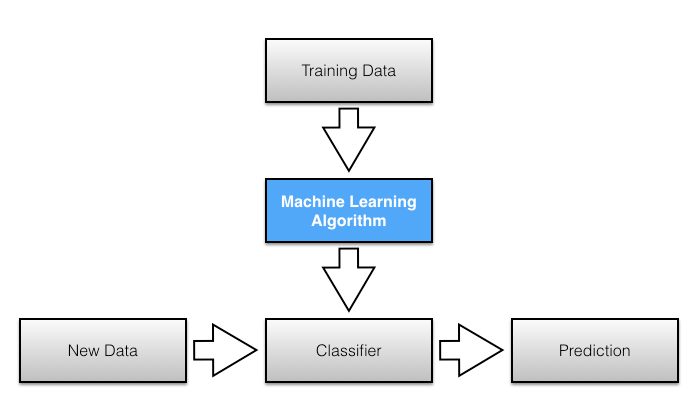
\includegraphics[width=15cm]{ml-uml}  
		\caption{\label{fig:uml-diagram} Diagrama generalp a algoritmului de învățare supervizată
		\protect
		\cite{ml_intro}}
	\end{figure}


	\newpage
	
	Modul de funcționare al algoritmilor de învățare automată este dat de clasificarea lor in cele doua tipuri, învățare supervizată si învățare nesupervizată. Punctul cheie care face diferența între aceste doua tipuri de algoritmi, este aprovizionarea învățării cu clase de clasificare și date de validare, in cazul invățării supervizate. Algoritmul învățării nesupervizate este bazat pe un curs “instinctiv” i.e. modalitatea de clasificare si împărțire este lăsata la latitudinea mașinii.
	
	Învățarea automată supervizată este bazată pe perechi alcătuite din date de intrare și o “etichetă” atribuită fiecărei date de intrare. Algoritmul va modela o funcție, bazată pe aceste perechi de intrare, iar scopul final este de a atribui corect unei valori arbitrare, nefamiliară algoritmului, o etichetă corespunzatoare din cele care i-au fost aprovizionate in etapa de invățare. 
	În contrast, invățarea automată nesupervizată este bazată doar pe date de intrare, astfel algoritmul fiind obligat să gestioneze informația fără a fi îndrumat. Avantajul acestui algoritm este faptul că poate gestiona probleme complexe, superioare creierului uman, prin faptul că va crea sau va atribui clase unor grupuri de date de intrare, bazat pe similarități descoperite pe parcurs.
	Alegerea tipului de învățare va fi dată de complexitatea si structura  datelor de intrare cât și de scopul problemei. Nu este exclusă posibilitatea utilizării celor doua metode concomitent, adeseori ducând la rezultate mai concise.
	
	\subsection{Aplicabilitate}
	Învățarea automată se regăsește în multe activități ale societății moderne, se extinde pe diferite planuri si acoperă nevoi de zi cu zi ale oamenilor. De la sugestii pe site-uri de muzică si clipuri video, filtrarea reclamelor si a conținutului de pe site-uri de socializare  si până la mașini cu funcționalitate de parcare automată, învățarea automată este raspunsul problemelor de gestionare și clasificare a evenimentelor și a stimulilor externi. 
	Învîțarea automată se întinde pe diferite domenii acoperind nevoi de bază dar excelând și în aplicații mai complexe.
	
	Printre domeniile în care inteligența artificială și invățarea automată și-au lăsat amprenta, se enumeră:
	
	\begin{itemize}
		\item Mașini inteligente. Învățarea automată, împreună cu senzorii de pe mașini, au adus o multitudine de functionalităti utile. Astăzi mașinile se pot parca și conduce singure și pot evita un accident iminent.
		
		\item Securitatea datelor. Virușii de tip Malware sunt o problemă persistentă din punctul de vedere al datelor personale ce prezintă o valoare pentru un atacator. Învățarea automată ajută în combaterea acestei probleme prin depistarea fișierelor de tip malware, noi apărute.
		
		\item Tranzacții financiare. Învățarea automată este folosită de mulți giganți ai pieței de capital și bursă, pentru realizarea unor schimburi automatizate căt mai precise
		
		\item Sănătate. Algoritmii predictivi sunt astăzi un factor important in detectarea precoce a unor probleme de sănătate, cum ar fi cancerul.
		
		\item Detectarea de fraude bancare. Bazat pe învățarea automată, băncile pot detecta când are loc o trănzacție fraudulentă sau spălare de bani, bazat pe detaliile acelei tranzacții.			
	\end{itemize}
	
	\vfill
	
	
	\section{Procesarea de imagini}
	Domeniul procesării de imagini nu poate fi definit sau clasificat printr-o simplă categorie. Acesta a fost si este intr-o continuă dezvoltare si urmăreste mai multe planuri. 
	
	Importanța acestor imagini digitale, se poate resimți pe multe domenii. Bazat pe aceste reprezentări și pe abilități dobândite până în prezent în materie de procesare și prelucrare, am obținut diferite rezultate si aplicabilități
	
	\subsection{Problema procesarii imaginilor}
	Problema procesării imaginilor se rezuma la procesul de învîțare a unui sistem cu abilităti pseudo-cognitive de a lua decizii pe baza unor detalii sau a unor caracteristici ale imaginii. Sistemul poate fi învățat, prin intermediul algoritmilor, să extragă caracteristici spre a le refolosi, sau poate utiliza date deja existente in scopul găsirii unor similarități. 
	
	Există diferite reprezentări ale imaginilor pe sisteme, definite ca și fiind formaturi. Unitatea de baza a imaginii este pixel-ul. Pixel este o prescurtare provenită de la Picture Element, și reprezintă un punct de la o poziție x, y a ecranului. În funcție de format, pixelul reprezintă proprietăți ale elementului de pe pozitia x, y; astfel de proprietăți pot fi culoarea și opțional, opacitatea elementului. O multitudine de pixel, fiecare cu proprietățiile proprii, reprezintă reprezentarea unei imagini. \cite{image_representation}
	
	\subsection{O noua perspectivă. Rețele Neuronale}
	Studiul creierului uman și a modului său de funcționare a deschis porți noi în domeniul științei. Felul în care neuronii comunică prin sinapse și iși întăresc legăturile cele mai des folosite, a inspirat oamenii de știință în creare unei analogii in domeniul științific, care va avea să rezolve probleme asemănătoare celor pe care creierul le gestionează.
	
	In 1943, idea unei  lucrări care prezenta modul de funcționare a creierului, semnată de  neurofiziologul Warren McClulloch și matematicianul Walter Pitts,   a fost susținută practic prin simularea funcțiilor neuronilor si a legăturile dintre ei, prin circuite electrice. Rețelele neuronale fizice, reprezentate prin circuite electrice, au fost primul stimulent care a introdus o nouă perspectivă în rezolvarea problemelor încă din înaintea dezvoltării domeniului inteligenței artificiale. 
	
	
	Rețelele neuronale artificiale au ca unitate de bază neuronul artificial, care primește unul sau mai multe semnale de intrare (asociate cu potențialul postsinaptic excitator și potențialul postsinaptic inhibator), care insumate vor rezulta un semnal de ieșire. Acest semnal de ieșire este mai apoi trecut printr-o funcție de activare (funcție de transfer) pentru a combate rezultatul linear al insumării semnalelor de intrare ale neuronului. (Vezi Fig. \ref{fig:neuron-schema})
	
	\begin{figure}[H]
		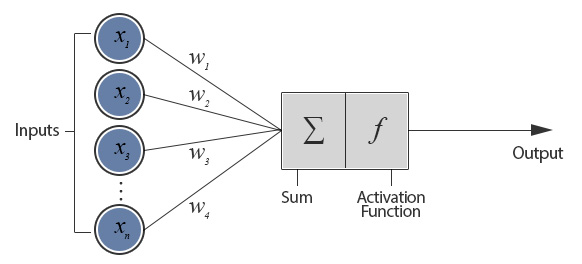
\includegraphics[width=15cm]{neuron-schema}  
		\caption{\label{fig:neuron-schema} Diagramp neuron artificial 
		\protect 
		\cite{ann}}
	\end{figure}
	
	
	Un model predictiv de rețele neuronale este alcătuit din mai multe straturi de neuroni, lucrând împreună pentru o modela o funcție non-lineară complexă.
	Fiecare strat va avea propriile proprietăți, cum ar fi: numărul de neuroni, ponderile aferente și funcția de activare.
	
	Procesul in care datele sunt procesate, prin straturile intermediare de neuroni, se numește operație feed-forward. La finalul operației feed-forward, algoritmul va prezenta datele asupra cărora s-a aplicat o mutație. Pe baza acestor date, algoritmul va verifica rezultatul obținut comparăndu-l cu un set de date de antrenare. 
	
	Odata ce eroare a fost obținută, aceasta va circula in sens invers prin straturile de neuroni și va ajusta ponderile ce au influențat decizia luată de model.
	
	

\end{document}